\section{\bench: a memory-dependent harvesting benchmark}
\label{sec:benchmark}

\subsection{Procedural orchard scene}
\bench\ is built on ManiSkill3 \citep{tao2025maniskill3} (environment \texttt{FruitPick-v1}). Each episode samples a tree with a trunk, branches and leaf clusters, and 4--6 spherical fruits of radius 2.5--2.9~cm. Fruits hang at heights of 0.44--0.64~m, at distances of 0.38--0.50~m from the robot base and within $\pm 28^\circ$ of azimuth. The layout sampler guarantees that each fruit has a horizontal-approach inverse-kinematics solution, that no branch blocks its approach corridor, and that fruits do not occlude each other in the front camera. A fruit is kinematically attached to its stem until it has been held between both fingers for two consecutive control steps; it then becomes a dynamic rigid body. Training, validation and test seeds are drawn from disjoint ranges.

\subsection{Robot and sensing}
The robot is a RealMan RM75-B 7-DoF arm with an EG2 parallel gripper under joint-position control (a 6-DoF RM65-B is also supported). Observations are a front camera and a wrist camera (both RGB-D, $256\times256$ pixels; the front camera has a $55^\circ$ field of view) and an 8-dimensional state (seven joint angles and one finger position). Actions are seven absolute joint targets and a gripper command.

\subsection{Tasks}
\label{sec:tasks}
Figure~\ref{fig:scene} shows both tasks.
\begin{itemize}
\item \textbf{FruitOccludedRipe.} Red (ripe) and green (unripe) fruits hang together. During a 30-step observation phase, a gust between steps 8 and 20 blows two leaf clusters in front of two fruits, at least one of them ripe, so ``hidden'' does not imply ``ripe''. The instruction is to put all ripe fruits into the basket. Leaves are pushed aside when the gripper comes within 15~cm, so the final approach is visible, but \emph{finding} a hidden ripe fruit requires remembering it. Success: every ripe fruit in the basket and no unripe fruit in it. Failure: an unripe fruit in the basket or a fruit dropped.
\item \textbf{FruitCount.} All $M$ fruits are ripe, and the instruction asks for exactly $N<M$ of them, with $N$ varying per episode (2--5). The basket is outside the front camera view, so the policy can only know how many it has picked by remembering its own picks. Success: exactly $N$ fruits in the basket. Failure: more than $N$ in the basket or a fruit dropped.
\end{itemize}

\begin{figure}[t]
\centering
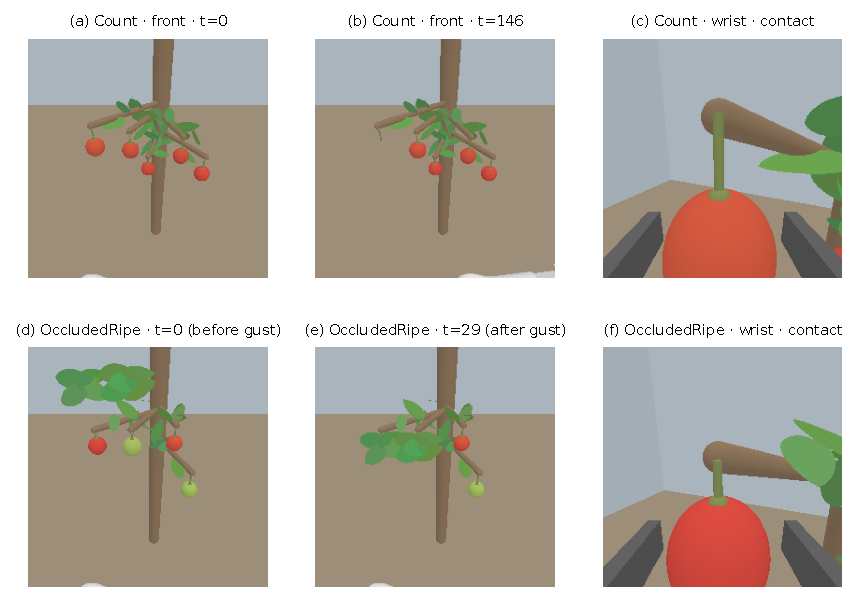
\includegraphics[width=\linewidth]{fig2_scene}
\caption{\bench\ tasks. (a--c) FruitCount: front view at the start and after one pick, and the wrist view at contact. (d--f) FruitOccludedRipe: the front view before and after the wind gust (two leaf clusters now hide fruits) and the wrist view at contact.}
\label{fig:scene}
\end{figure}

\subsection{Demonstrations}
A scripted demonstrator plans with mplib \citep{mplib} through eight phases: observe, reach, approach, grasp, pull, carry, release and settle. An attempt that fails (planning failure, no detachment, missed basket, task not completed) is discarded and the seed is advanced, so only successful demonstrations are kept. Every frame stores the simulator ground truth: fruit poses and attachment, visible pixel counts per camera, phase labels and the TCP pose. Recovery demonstrations (DART-H, Section~\ref{sec:dart}) use the same demonstrator with execution noise.

Table~\ref{tab:dataset} summarizes the 640 demonstrations: 200 clean training, 200 DART-H training, 40 development (used only for a go/no-go gate) and 200 validation episodes. Table~\ref{tab:occlusion} quantifies occlusion. After the gust, the targeted fruits are fully invisible in the front camera. Over all frames in which an occluded fruit is still on the tree, it is invisible in 72\% of frames on average (median 78\%). Remembering where it is, rather than seeing it, is therefore a precondition for picking it.

\begin{table}[t]
\centering
\caption{Benchmark statistics (mean $\pm$ SD [min, max]). Acceptance: fraction of demonstrator attempts that succeeded.}
\label{tab:dataset}
\small
\begin{adjustbox}{max width=\textwidth}\begin{tabular}{llrcccc}
\toprule
Set (episodes) & Task & $n$ & Steps & Fruits & Picks & Acceptance\\
\midrule
Clean train (0--99) & FruitCount & 100 & $474\pm124$ [320, 757] & 4.73 & 2.85 & 0.96\\
 & FruitOccludedRipe & 100 & $412\pm85$ [295, 710] & 4.69 & 2.54 & 0.98\\
DART-H train (100--199) & FruitCount & 100 & $455\pm133$ [314, 876] & 4.62 & 2.70 & 0.57\\
 & FruitOccludedRipe & 100 & $397\pm89$ [297, 672] & 4.78 & 2.46 & 0.66\\
Development (200--219) & FruitCount & 20 & $487\pm162$ [321, 766] & 5.05 & 3.10 & 1.00\\
 & FruitOccludedRipe & 20 & $369\pm71$ [300, 471] & 4.60 & 2.35 & 0.95\\
Validation (0--49) & FruitCount & 50 & $459\pm142$ [314, 904] & 4.58 & 2.82 & 0.98\\
 & FruitOccludedRipe & 50 & $396\pm87$ [300, 630] & 4.72 & 2.50 & 0.96\\
Validation (50--99) & FruitCount & 50 & $499\pm169$ [322, 1037]$^{a}$ & 4.67 & 2.98 & 0.91\\
 & FruitOccludedRipe & 50 & $392\pm73$ [304, 534] & 4.54 & 2.52 & 0.98\\
\bottomrule
\end{tabular}\end{adjustbox}

\footnotesize $^{a}$Statistics over 49 episodes; the ground-truth file of one episode was regenerated after these statistics were computed. Training features: 88,607 samples (clean) and 173,791 samples (clean + DART-H).
\end{table}

\begin{table}[t]
\centering
\caption{Occlusion and phase structure (clean training set).}
\label{tab:occlusion}
\small
\begin{adjustbox}{max width=\textwidth}\begin{tabular}{lc}
\toprule
Quantity & Value\\
\midrule
Leaf clusters per FruitOccludedRipe episode & 2 (66\% hide a ripe fruit)\\
Occluded fruits fully invisible in the front camera after the gust & 100\%\\
Frames (fruit still on tree) in which an occluded fruit is invisible & mean 72\%, median 78\%\\
Visible fraction of non-occluded fruits after the gust (median) & 1.00\\
Ripe / unripe fruits per FruitOccludedRipe episode & 2.54 / 2.15\\
Mean steps per phase, FruitCount (observe / reach / approach / grasp / & 30 / 118 / 59 / 29 /\\
\quad pull / carry / release / settle) & 58 / 117 / 23 / 34\\
\bottomrule
\end{tabular}\end{adjustbox}
\end{table}
